%!TEX root = thesis.tex

\chapter{Component-Based Garbled Circuits}

In this chapter we introduce component-based garbled circuits, a method that allows for most of the work involved in building and communicating a garbled circuit to occur in an offline phase before the inputs or function to compute are known. 
This offers significant improvements to the online performance of garbled circuits. 

Component-based garbled circuits are the research of a larger project to which this thesis contributes. 
The first part of this chapter will describe naive component-based garbled circuits. 
Naive component-based garbled circuits are presented in an unpublished paper, and I am a coauthor on the paper. 
I contributed two items to the unpublished paper.
The first is an improvement to component-based garbled circuits called single communication multiple connections (SCMC); we present SCMC at the end of this chapter. 
The second is \CompGC, an implementation of component-based garbled circuits. 
We discuss \CompGC in detail in Chapter 5. 

\section{History}
The goal to reduce online computation by using an offline phase is not a new goal.
In Chapter 3, we discuss oblivious transfer preprocessing, a method that moves most of the work involved in oblivious transfer to an offline stage \cite{Bea95}. 
In the research of malicious garbled circuits, researchers improve the online efficiency of cut-and-choose by using an offline phase \cite{HKK14, LR14, blazing-fast}.
Moreover, research in non-garbled circuit two party computation uses similar ideas in \cite{DPSZ12, NNOB12}. 

Most similar to component-based garbled circuits is a technique called \textit{partial garbled circuits} proposed by Mood et al. \cite{MGBF14}. 
The goal of partial garbled circuits was to retain state after a garbled circuit computation. 
To achieve this, Mood et al. use two link labels per connection, whereas we use fewer than one label per connection on average.   

\section{Naive Component-Based Garbled Circuits}
Component-based garbled circuits begin with the observation that most functions are composed of many smaller components. 
For example, many statistical operations are a composition of matrix operations; Smith-Waterman and Levenshtein distance, two algorithms important to analyzing genomes, are dynamic programs that run a single procedure inside a \textit{for} loop; and encrypting arbitrary length messages via modes of operation repeats the encryption algorithm a number of times.
The gist of component-based garbled circuits is then to build and communicate many small, garbled components in the offline stage.
Later, in the online stage, the garbler and evaluator combine the pre-communicated components to form a larger function. 
They compute each component individually, linking wire labels from one component to another as needed. 

Imagine that two banks integrate secure computation into their daily transactions.
At night when activity is low, the banks' servers exchange many garbled circuits, and then during the day, they use the pre-exchanged garbled circuits to quickly perform secure computation.
The computational requirements for the banks, when they compute the function, is to exchange input labels and for the evaluator-bank to evaluate the garbled circuit, while, importantly, the banks preserve the ability to choose their inputs and the function to be computed at the time of the computation. 

%!TEX root = thesis.tex


\begin{figure}
\centering
                        \scalebox{1.0}{
                            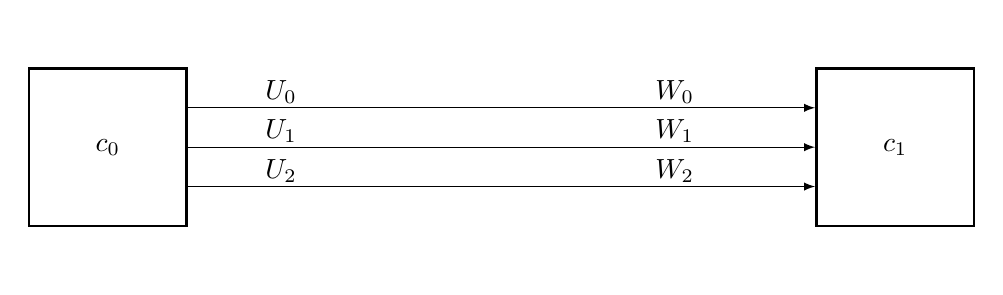
\begin{tikzpicture}
                                [
                                    square/.style = {draw, shape=rectangle, minimum height=2cm, minimum width=2cm, node distance=2cm, line width=1pt},
                                    empty/.style = {draw, shape=rectangle, minimum height=2cm, minimum width=2cm, node distance=2cm, line width=1pt, draw=white},
                                ]

                                \node[empty] (0a) at (0,0.5)     {};
                                \node[empty] (0b) at (0,-0.5)     {};
                                \node[square] (0c) at (0,0)     {$c_0$};

                                \node[empty] (1a) at (10cm,0.5)   {};
                                \node[empty] (1b) at (10cm,-0.5)   {};
                                \node[square] (1c) at (10cm,0)   {$c_1$};

                                \node (x0) at (2.2cm,0.7) {$U_0$};
                                \node (y0) at (2.2cm,-0.3) {$U_2$};
                                \node (z0) at (2.2cm,0.2) {$U_1$};

                                \node (x1) at (7.2cm,0.7) {$W_0$};
                                \node (y1) at (7.2cm,-0.3) {$W_2$};
                                \node (z1) at (7.2cm,0.2) {$W_1$};

                                \draw [-latex] (0a.east) -- (1a.west);
                                \draw [-latex] (0b.east) -- (1b.west);
                                \draw [-latex] (0c.east) -- (1c.west);
                            \end{tikzpicture}
                            
                        }
                        \caption{An example of linking component $c_0$ to component $c_1$. The output wires of $c_1$, $U_0, U_1$ and $U_2$, are linked to the input wires of $c_1$, $W_0, W_1$ and $W_2$.}
                            \label{fig:chaining}
                    \end{figure}
                    
                    
                    %!TEX root = thesis.tex
%
%
%\begin{figure}
%\centering
%                        \scalebox{1.0}{
%                            \begin{tikzpicture}
%                                [
%                                    square/.style = {draw, shape=rectangle, minimum height=2cm, minimum width=2cm, node distance=2cm, line width=1pt},
%                                    empty/.style = {draw, shape=rectangle, minimum height=2cm, minimum width=2cm, node distance=2cm, line width=1pt, draw=white},
%                                ]
%
%                                \node[empty] (0a) at (0,0.5)     {};
%                                \node[empty] (0b) at (0,-0.5)     {};
%                                \node[square] (0c) at (0,0)     {$c_0$};
%
%                                \node[color=blue] (mida) at (4.8cm,0.5)   {$A \oplus X$};
%                                \node[color=blue] (midb) at (4.8cm,-0.5)  {$C \oplus Z$}; 
%                                \node[color=blue] (midc) at (4.8cm,0)     {$B \oplus Y$};
%
%                                \node[empty] (1a) at (10cm,0.5)   {};
%                                \node[empty] (1b) at (10cm,-0.5)   {};
%                                \node[square] (1c) at (10cm,0)   {$c_1$};
%
%                                \node (x0) at (2.2cm,0.7) {$U_0$};
%                                \node (y0) at (2.2cm,-0.3) {$U_2$};
%                                \node (z0) at (2.2cm,0.2) {$U_1$};
%
%                                \node (x1) at (7.2cm,0.7) {$W_0$};
%                                \node (y1) at (7.2cm,-0.3) {$W_2$};
%                                \node (z1) at (7.2cm,0.2) {$W_1$};
%
%                                \draw [-latex] (0a.east) -- (mida.west);
%                                \draw [-latex] (0b.east) -- (midb.west);
%                                \draw [-latex] (0c.east) -- (midc.west);
%
%                                \draw [-latex] (mida.east) -- (1a.west);
%                                \draw [-latex] (midb.east) -- (1b.west);
%                                \draw [-latex] (midc.east) -- (1c.west);
%                            \end{tikzpicture}
%                        }
%                    \end{figure}

At a coarse level, chaining looks like figure \ref{fig:chaining} where the input to some some garbled components is the output of other garbler components. 
To chain, or stitch together, two garbled components, the evaluator needs to transform an output wire label of one component into a valid input wire label of another component, while preserving the semantic value of the wires. 
In figure \ref{fig:chaining} the zeroth output wire of $c_0$, $U_0$, needs to transform into the zeroth input wire of $c_1$, $W_0$. 
We specifically desire that the evaluator transforms $U_0^0$ into $W_0^0$ and $U_0^1$ into $W_0^1$. 

%!TEX root = thesis.tex

\begin{figure}
\centering
                        \scalebox{1.0}{
                            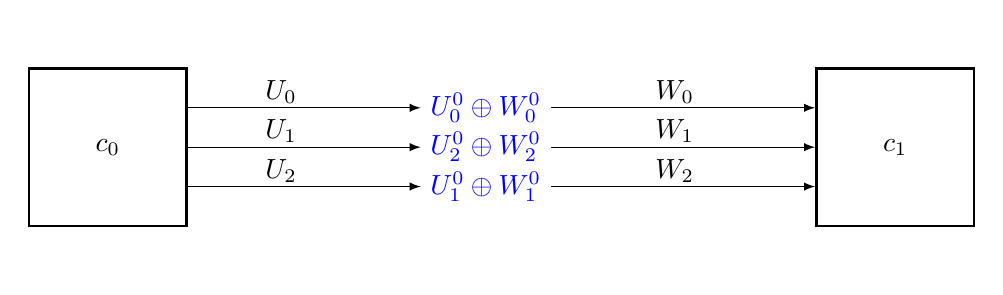
\begin{tikzpicture}
                                [
                                    square/.style = {draw, shape=rectangle, minimum height=2cm, minimum width=2cm, node distance=2cm, line width=1pt},
                                    empty/.style = {draw, shape=rectangle, minimum height=2cm, minimum width=2cm, node distance=2cm, line width=1pt, draw=white},
                                ]

                                \node[empty] (0a) at (0,0.5)     {};
                                \node[empty] (0b) at (0,-0.5)     {};
                                \node[square] (0c) at (0,0)     {$c_0$};

                                \node[color=blue] (mida) at (4.8cm,0.5)   {$U_0^0\oplus W_0^0$};
                                \node[color=blue] (midb) at (4.8cm,-0.5)  {$U_1^0 \oplus W_1^0$}; 
                                \node[color=blue] (midc) at (4.8cm,0)     {$U_2^0 \oplus W_2^0$};

                                \node[empty] (1a) at (10cm,0.5)   {};
                                \node[empty] (1b) at (10cm,-0.5)   {};
                                \node[square] (1c) at (10cm,0)   {$c_1$};

                                \node (x0) at (2.2cm,0.7) {$U_0$};
                                \node (y0) at (2.2cm,-0.3) {$U_2$};
                                \node (z0) at (2.2cm,0.2) {$U_1$};

                                \node (x1) at (7.2cm,0.7) {$W_0$};
                                \node (y1) at (7.2cm,-0.3) {$W_2$};
                                \node (z1) at (7.2cm,0.2) {$W_1$};

                                \draw [-latex] (0a.east) -- (mida.west);
                                \draw [-latex] (0b.east) -- (midb.west);
                                \draw [-latex] (0c.east) -- (midc.west);

                                \draw [-latex] (mida.east) -- (1a.west);
                                \draw [-latex] (midb.east) -- (1b.west);
                                \draw [-latex] (midc.east) -- (1c.west);
                            \end{tikzpicture}
                        }
                        \caption{An example of linking component $c_0$ to component $c_1$. The link labels for linking the output wires of $c_0$ and the input wires of $c_1$ are shown between the wires in blue.}
                        \label{fig:chaining2}
                    \end{figure}

To achieve this transformation, the garbler sends the evaluator a link label.
A link label is a ciphertext that allows the evaluator to transform the output wire label into the appropriate input wire label. 
Suppose that the garbling scheme uses Free XOR where each component uses the same $\Delta$, that is, $U_0^0 \oplus U_0^1 = W_0^0 \oplus W_0^1 = \Delta$, then it is sufficient for the link label $L_{UW}$ to be $U_0^0 \oplus W_0^0$.
The evaluator xors the output wire label $U_0^*$ with $L_{UW}$ to acquire $W_0^*$, a valid wire label for wire $W_0$. 

We show this computation below; the value $u_0 \in \{0,1\}$ is the semantic value of wire $U_0$.
For information on this notation, see section 3.5. 
\begin{align}
	U_0^0 \oplus u_0 \Delta \oplus L_{UW} & = U_0^0 \oplus u_0 \Delta \oplus U_0^0 \oplus W_0^0 \\
	& = W_0^0 \oplus u_0 \Delta
\end{align}
We see from this equation that the evaluator acquires a valid wire label for wire $W_0$ which has the same semantic value as wire label $U_0^*$.

We formally describe component-based garbled circuits as a tuple of three algorithms $(\Garble, \Link, \Eval)$.
The $\Garble$ algorithm is the same algorithm that we used before to garble circuits; it takes as inputs a circuit $\C$ and outputs three pieces of information: a garbled circuit $\GC$, a set of input wires $e_{\C}$, and a set of output wires $d_{\C}$.
In the component-based setting, the $\Garble$ algorithm can also take a component-circuit $c$ as input, to which the algorithm outputs a garbled component $\GC_c$, input wire set $e_c$ and output wire set $d_c$. 

The $\Link$ algorithm is unique to component-based garbled circuits, and it produces the link labels necessary for linking.
$\Link$ takes as input two garbled components $c_0 = (\GC_0, e_0, d_0)$ and $c_1 = (\GC_1, e_1, d_1)$, and a mapping of output wires of $c_0$ to input wires of $c_1$. 
$\Link$ outputs the \textit{link} labels needed to convert the output wires $d_0$ to input wires $e_1$. 
Suppose that output wire $U_i \in d_0$ has labels $(U_i^0, U_i^1)$, and input wire $W_j \in e_1$ has wire labels $(W_j^0, W_j^1)$, then $\Link$ outputs $L_{u_i w_j} = U_i^0 \oplus W_j^0$. 
The discussion above explains why link label $L_{u_i w_j}$ is sufficient for linking. 

The $\Eval$ algorithm evaluates the garbled components and links garbled circuits where necessary.
It takes three inputs: a list of a garbled components $\{c_i\}$, linking labels $\{L_{ij}\}$ and input labels $\{W_i\}$, and it outputs output labels $\{Z_i\}$. 
$\Eval$ starts with the inputs, and then proceeds component by component, evaluating each component in order to get the component output wire labels.
Where necessary, $\Eval$ uses component output wire labels and link labels to compute the appropriate input wire label for later components. 
Once all components are evaluated, $\Eval$ recovers the garbled outputs $\{Z_i\}$ from the output components, and uses $d$ for that component to recover the real output $y$. 

Let us think about how the two banks who use secure computation in their daily operations employ the three algorithms.
At night, during the offline stage, the garbler-bank generates many circuit components, garbles them with $\Garble$, and sends the garbled circuits to the other evaluator-bank. 
The garbler-bank and evaluator-bank also perform the offline phase of OT-preprocessing.
During the day, when the banks decide that they want to securely compute some function $f$, the garbler-bank runs $\Link$ on the components used in $f$ to generate the link labels, which the garbler-bank subsequently sends to the evaluator-bank.
The garbler-bank and evaluator-bank also exchange wire labels, some via online OT-preprocessing. 
Now that the evaluator-bank has the garbled components, link labels and input labels, they run $\Eval$, recovering the output of the function.

\section{Security of Component-Based Garbled Circuits}

In this section, we show how to adapt the standard definition of privacy, presented in chapter 2, to component-based garbled circuits.
Recall from Chapter 2 that we said a garbled circuit scheme is secure if for all probabilistic, polynomial-time simulators (i.e algorithms) $S_1$ and $S_2$ the following holds:
\begin{equation}
\label{eqn:party1}
    \{(S_1(x, f_1(x,y), f(x,y)))\}_{x,y} \compindist \{(\viewrv^{\Pi}_1(x,y), \outputrv^{\Pi}(x,y)) \}_{x,y}
\end{equation}
\begin{equation}
\label{eqn:party2}
    \{(S_2(x, f_2(x,y), f(x,y)))\}_{x,y} \compindist \{(\viewrv^{\Pi}_2(x,y), \outputrv^{\Pi}(x,y)) \}_{x,y}
\end{equation}

To consider the security of component-based garbled circuits, we add in the extra information that each party receives into $\viewrv^{\Pi}(x,y)$. 
Party 1, the garbler, only receives additional information from OT-preprocessing, which we know to be secure, hence equation \ref{eqn:party1} remains true. 

We think through the security of the evaluator, party 2, using \textit{hybrids}, a common cryptographic technique in proofs. 
A hybrid argument begins by imagining the protocol in the real world. 
The aim is to show that the real world protocol is computationally indistinguishable from the ideal world. 
To achieve this, we rely on the fact that computational indistinguishability is transitive, that is if for worlds $X, Y$ and $Z$ such that $X \compindist Y \compindist Z$, we know that $X \compindist Z$. 
The hybrid argument starts with the real world and makes a small incremental change to make it more similar to the ideal world.
Then we take the modified world and make another small change such that it is more similar to the ideal world. 
Eventually, the world that we are operating with is the ideal world. 
If at every step, we prove that the previous world is computationally indistinguishable from the next world, then by the transitivity of computationally indistinguishability, we have shown that the real world is computationally indistinguishable from the ideal world. 

We start with the real world protocol, in which the evaluator has the following information: pre-garbled components $\{GC_i\}_{i = 0}^{|\Components|}$, input labels $\{W_j^{x_j}\}_{j \in \Inputs(C)}$, output map $d_{C_{out}}$ and link labels $\{L_{ij}\}_{i,j \in \Components}$.
We first suppose that the garbler, instead of sending correct link labels, sends garbage, random values for link labels. 
Yes, this will prevent Bob from recovering the correct output, but correctness is irrelevant when we are reasoning about security; we are only concerned with the information that Bob can infer. 
We now ask the question: is the real world computationally indistinguishable from the world where Bob receives incorrect link labels?
Or worded more accessibly: does Bob learn any more information from correct wire labels than he does from garbage wire labels?
We argue, without proof, that Bob does not learn any more information because (1) the link labels are encrypted so they look like garbage to Bob anyways, and (2) Bob cannot use the link labels with other pieces of data, such as input wire labels of the garbled circuits, to gain information. 

We now hybrid from the world in which Bob receives garbage link labels to a world in which Bob receives both garbage link labels and garbage input wire labels. 
Again, we note that Bob will not recover the correct answer, but correctness is irrelevant to our aim. 
We know that input wire labels do not give Bob any information from our proof in Chapter 3 that garbled circuits are secure. 
Therefore these two worlds are computationally indistinguishable. 

By referencing the proof in Chapter 3 that garbled circuits are secure, we also know that turning the output map and garbled circuits into garbage values gives Bob no more information.
This means a world in which all the information that Bob receives is garbage is computationally indistinguishable from the real world.
This garbage infested world is identically the ideal world - the only non-garbage value Bob has is his input, just like the ideal world - hence we successfully argue that the real world is computationally indistinguishable from the ideal world, satisfying equation \ref{eqn:party2}. 

It should be noted that this not even close to a formal proof of security.
A formal proof is long, many pages long, and beyond the scope of this project; rather, this section highlights the intuition behind why we believe a formal proof of security to be possible. 

\section{Single Communication Multiple Connections}

At the begining of my thesis project, I was presented naive component-based garbled circuits, and I was asked to implement the ideas in a program (see Chapter 5) as part of a larger research project. 
In this midst of writing the program, I discovered a method to improve the efficiency of chaining. 
In this section I discuss my theoretical contribution to component-based garbled circuits:  \textit{single communication multiple connections}.

Single communication multiple connections (SCMC) is a technique that improves upon naive component-based garbled circuits for some functions by observing that large sequences of consecutive wires often represent a single element of data, like a string, number or matrix. 
When large sequences of consecutive wires are mapped between garbled components, the sequence of consecutive wires is mapped together - the order of the wires is preserved. 
SCMC takes advantage of this fact by requiring that only a single link label is communicated for each sequence of consecutive wires, as opposed to one link label per wire. 
This technique is analogous to SIMD-style (single instruction multiple data) computation that is used in homomorphic encryption \cite{SV11} and GMW-based two party computation \cite{DSZ15, SZ13} in that a single piece of communication, or a single instruction, is used for multiple links, or data. 

As with most improvements to garbled circuits, SCMC operates by modifying the generation of wire labels. 
Wire labels that are part of a block representing a single piece of data are generated in a fixed, patterned way such that the differences between linked labels will be the same for all wires in a block. 

SCMC modifies the $\Garble$ algorithm by choosing input wires and output wires in a particular way. 
For every component, we first choose three random labels $A,B$ and $T$: $A$ and $B$ are the base values for input wires and output wires respectively, and $T$ is a tweak value, ensuring security for the random oracle.
We next assume that all parties have access to a random oracle $H$. 
A random oracle is a theoretically perfect random function, which on input of any value $x \in \{0,1\}^*$, returns a value from $\{0,1\}^{\lambda}$ selected uniformly at random.
In practice, we use a hash function for $H$. 
Then, for all input wire labels $W_i^b$, set wire label $W_i^b$ to $A \oplus H(T \oplus (i || b))$. 
Likewise, for all output wires labels $W_i^b$, we do the same process, setting $W_i^b$ to $B \oplus H(T \oplus (i || b))$.

Suppose that all output wires of component $c_0$ are being linked to the input wires component $c_1$, where the $i$th input wire is being mapped to the $i$th output wire. 
Then, it is sufficient for the garbler to send $B_{c_0} \oplus A_{c_1}$ to the garbler. 
This works since for any wire $i$ and bit $b$,
\begin{equation}
(B_{c_0} \oplus H(T \oplus (i || b)) \oplus (B_{c_0} \oplus A_{c_1}) = A_{c_1} \oplus H(T \oplus (i || b))
\end{equation}

Evaluation is the same as naive component-based garbled circuits, wherein the evaluator links using the correct wire label.

\subsection{Analysis}
SCMC substantially reduces the amount of communication required for chaining. 
For example, if AES is being computed where the components are single AES rounds, then SCMC requires only $9$ link labels to be communicated between the garbler and evaluator; in contrast, naive component-based garbled circuits requires $1152$ labels. 

The advantage gained from SCMC varies based on the function being computed and components being used. 
SCMC offers the most benefits to functions that are modular, and where large amounts of data are being passed around, like matrix-based functions and dynamic programs like Levenshtein distance. 
When using SCMC, online bandwidth does not scale with an increase in data size. 
SCMC requires that a single link label be communicated for a 2 by 2 matrix and for a 1,000 by 1,000 matrix. 
Thereby, SCMC greatly improves the speed of securely computing large statistical computations, such as those that might be performed by hospitals or on genomes. 

The security of SCMC follows directly from the security of naive component-based garbled circuits. 
The wire labels again do not offer any information, so a similar hybrid proof works in the SCMC setting as well. 
There is a caveat: SCMC uses a new method of generating wire labels. 
This is secure since $H$ is a random function, hence $H(\cdot)$ blinds $A$ and $B$; in particular, the wire labels are only distinguishable if the evaluator can determine $T$, which is not possible since $H$ is a random oracle.
Therefore, SCMC is secure. 
































